% Source for the figure of SellMatrix (sec. 17.7): the two chunks of C = 4
% rows of an 8-row matrix with sigma = 8; each column of a chunk is the
% k-th nonzero of its 4 rows, stored one after the other, and the faint
% places are the padding. Build: make figures (in ../build).
\documentclass[border=4pt]{standalone}
\usepackage[T1]{fontenc}
\usepackage{lmodern}
\usepackage{amsmath,amssymb}
\usepackage{tikz}
\usepackage{lamalunga}
% tikz-ads.tex: the TikZ styles shared by the figures of the memory of the
% manual, \input by each standalone figure: a cell of a vector (cell), the
% cell that an operation touches (touched), a free cell (free), a node of a
% linked structure (node), the labels of indices (index) and of variables
% (var), a pointer (ptr), and \cells and \indices to draw a row of cells.
\usetikzlibrary{arrows.meta,positioning,calc,fit,shapes.multipart}
\definecolor{adsTouched}{RGB}{214,196,236}
\definecolor{adsFree}{RGB}{236,236,236}
\tikzset{
  ads/.style={>={Stealth[length=2mm]},font=\small,
              every node/.append style={inner sep=0pt}},
  cell/.style={draw,minimum width=7mm,minimum height=7mm,
               font=\small\ttfamily,outer sep=0pt},
  touched/.style={cell,fill=adsTouched},
  free/.style={cell,fill=adsFree,text=black!45},
  node/.style={draw,rounded corners=1pt,minimum width=8mm,
               minimum height=6mm,font=\small\ttfamily},
  index/.style={font=\scriptsize\ttfamily,text=black!60},
  var/.style={font=\small\itshape},
  ptr/.style={->,thick}
}
% \cells{name}{x,y}{list}: a row of cells, the first at (x,y), named
% name-0, name-1, ...; each item is text/style, the style one of cell,
% touched and free (e.g., {a/cell,e/touched,/free})
\newcommand{\cells}[3]{%
  \foreach \v/\s [count=\i from 0] in {#3}
    \node[\s] (#1-\i) at ($(#2)+(\i*7mm,0)$) {\v};}
% \indices{name}{n}: the indices 0 .. n-1 under the cells of name
\newcommand{\indices}[2]{%
  \foreach \i in {0,...,\numexpr#2-1\relax}
    \node[index,below=1.2mm of #1-\i] {\i};}

\begin{document}
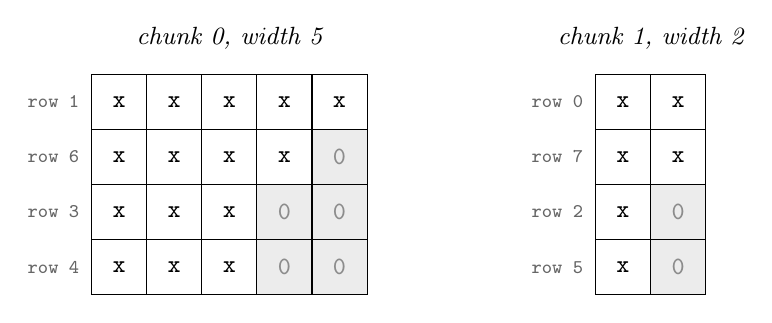
\begin{tikzpicture}[ads]
  % chunk 0: rows 1, 6, 3, 4 of lengths 5, 4, 3, 3
  \foreach \r/\len [count=\l from 0] in {1/5,6/4,3/3,4/3} {
    \node[index,anchor=east] at (-5mm,-\l*7mm) {row \r};
    \foreach \k in {0,...,4} {
      \ifnum\k<\len \node[cell] at (\k*7mm,-\l*7mm) {x};
      \else \node[free] at (\k*7mm,-\l*7mm) {0}; \fi } }
  % chunk 1: rows 0, 7, 2, 5 of lengths 2, 2, 1, 1
  \foreach \r/\len [count=\l from 0] in {0/2,7/2,2/1,5/1} {
    \node[index,anchor=east] at (59mm,-\l*7mm) {row \r};
    \foreach \k in {0,1} {
      \ifnum\k<\len \node[cell] at (64mm+\k*7mm,-\l*7mm) {x};
      \else \node[free] at (64mm+\k*7mm,-\l*7mm) {0}; \fi } }
  \node[var] at (14mm,8mm) {chunk 0, width 5};
  \node[var] at (67.5mm,8mm) {chunk 1, width 2};
\end{tikzpicture}
\end{document}
